\documentclass[crop, tikz]{standalone}

\usepackage{tkz-base}

\begin{document}
    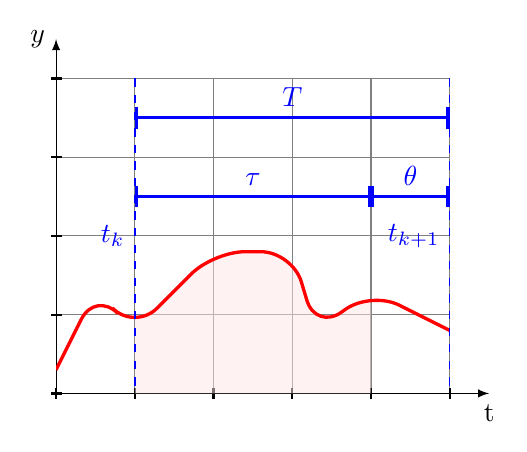
\begin{tikzpicture}
        \tkzInit[xmax=5,ymax=4,xmin=0]
        \tkzGrid
        \tkzDrawY \tkzDrawX[label=t]% \tkzLabelX \tkzLabelY
        \tkzClip
        \begin{scope}
            \clip (1,0) -- ++(0,2) -- ++(3,0) -- ++(0,-2) -- cycle;
            \fill[opacity=0.5, red!10] (0,0) -- (0,0.3) {[rounded corners=4mm] -- ++(0.5,1) -- ++(0.5,-0.5) -- ++(1,1) -- ++(1,0)  -- ++(0.3,-1) -- ++(0.7,0.5)} -- ++(1,-0.5) -- (5,0) -- cycle;
        \end{scope}
        \draw[very thick,red, rounded corners=4mm]
            (0,0.3) -- ++(0.5,1) -- ++(0.5,-0.5) -- ++(1,1) -- ++(1,0)  -- ++(0.3,-1) -- ++(0.7,0.5) -- ++(1,-0.5)
        ;
        \draw[|-|, blue, very thick] (1,3.5) --  ++(4,0) node [midway, above] {$T$};
        \draw[|-|, blue, very thick] (1,2.5) --  ++(3,0) node [midway, above] {$\tau$};
        \draw[|-|, blue, very thick] (4,2.5) --  ++(1,0) node [midway, above] {$\theta$};
        \draw[dashed, blue, thick] (1,4) --  ++(0,-4) node [midway, left] {$t_k$};
        \draw[dashed, blue, thick] (5,4) --  ++(0,-4) node [midway, left] {$t_{k+1}$};
    \end{tikzpicture}
\end{document}
